\documentclass[a4paper,12pt]{article}
\usepackage{graphicx}
\usepackage{float}
\usepackage{hyperref}
\usepackage{geometry}
\usepackage{polski} 

\geometry{margin=1in}

\title{Laboratorium 1}
\author{Łuszczek Patryk\\
        272707}
\date{\today}

\begin{document}

\maketitle

\section{Cel zadania}
Celem zadania było stworzenie aplikacji typu PWA - Progressive Web App oraz wdrożenie jej w system chmurowy.
Progressive Web App to aplikacja internetowa, która wykorzystuje możliwości nowoczesnych przeglądarek internetowych, aby zapewnić użytkownikom doświadczenie podobne do aplikacji natywnych. Aplikacje PWA są responsywne, szybkie i mogą działać offline, co czyni je idealnym rozwiązaniem dla użytkowników mobilnych.
\section{Opis aplikaci}
Aplikacja służy do proponowania przepisow kulinarnych pobieranych z API dostępnego pod adresem \texttt{https://www.themealdb.com}.
Użytkownik po wejściu do aplikacji może przeglądać losowo pobierane przepisy oraz zapisywać je do ulubionych. Przepisy zapisane do ulubionych są następnie przechowywane w pamięci, co pozwala na ich późniejsze przeglądanie nawet w trybie offline.

\section{Opis procesu}
\subsection{Tworzenie aplikacji}
W celu umożliwienia dzialaności aplikacji jako PWA został utworzony "service worker", który obsługuje cache'owanie zasobów aplikacji oraz zapewnienie możliwości działania offline.
W czasie instalacji aplikacji SW zapisuje do pamięci podręcznej zdefiniowane pliki, w tym przypadku były to pliki \texttt{index.html}, \texttt{style.css}, \texttt{main.js}.
Równie ważnym krokiem było utworzenie pliku manifestu, który definiuje podstawowe informacji aplikacji takie jak nazwa, ikona czy kolor motywu.

\begin{figure}[H]
    \centering
    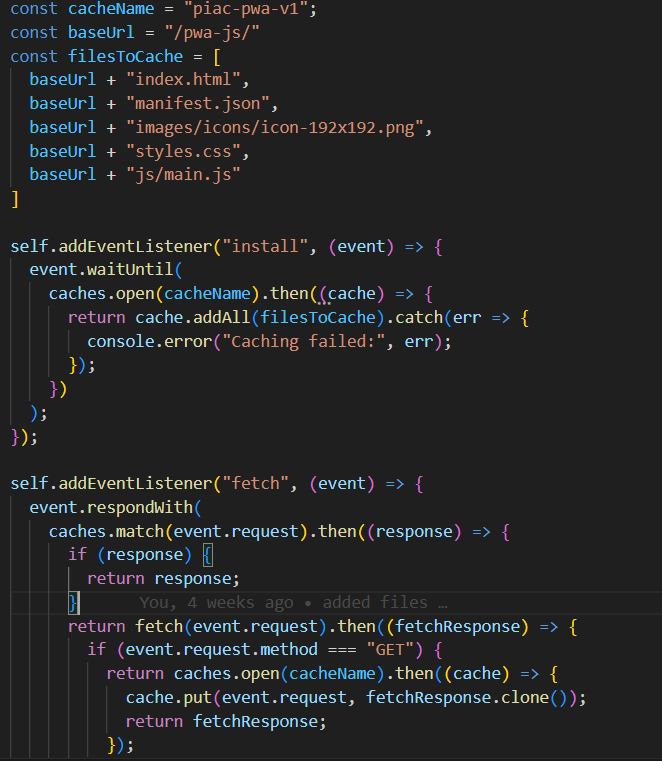
\includegraphics[width=0.5\textwidth]{images/sw.png}
    \caption{Service worker}
    \label{fig:sw}
\end{figure}

Dodatkowo w pliku \texttt{index.html} dodano odpowiednie tagi linkujące do pliku manifestu oraz zawierające ikony aplikacji wyświetlane na urządzeniach mobilnych.

\subsection{Wygląd, funkcjonalność i instalacja aplikacji}

Jak już wcześniej wspomniano, aplikacja służy do przeglądania nowych przepisów kulinarnych. Po wejściu do aplikacji pokazuje się splash screen, a następnie przedstawiany jest
losowy przepis (o ile jest dostęp do internetu).

\begin{figure}[H]
    \centering
    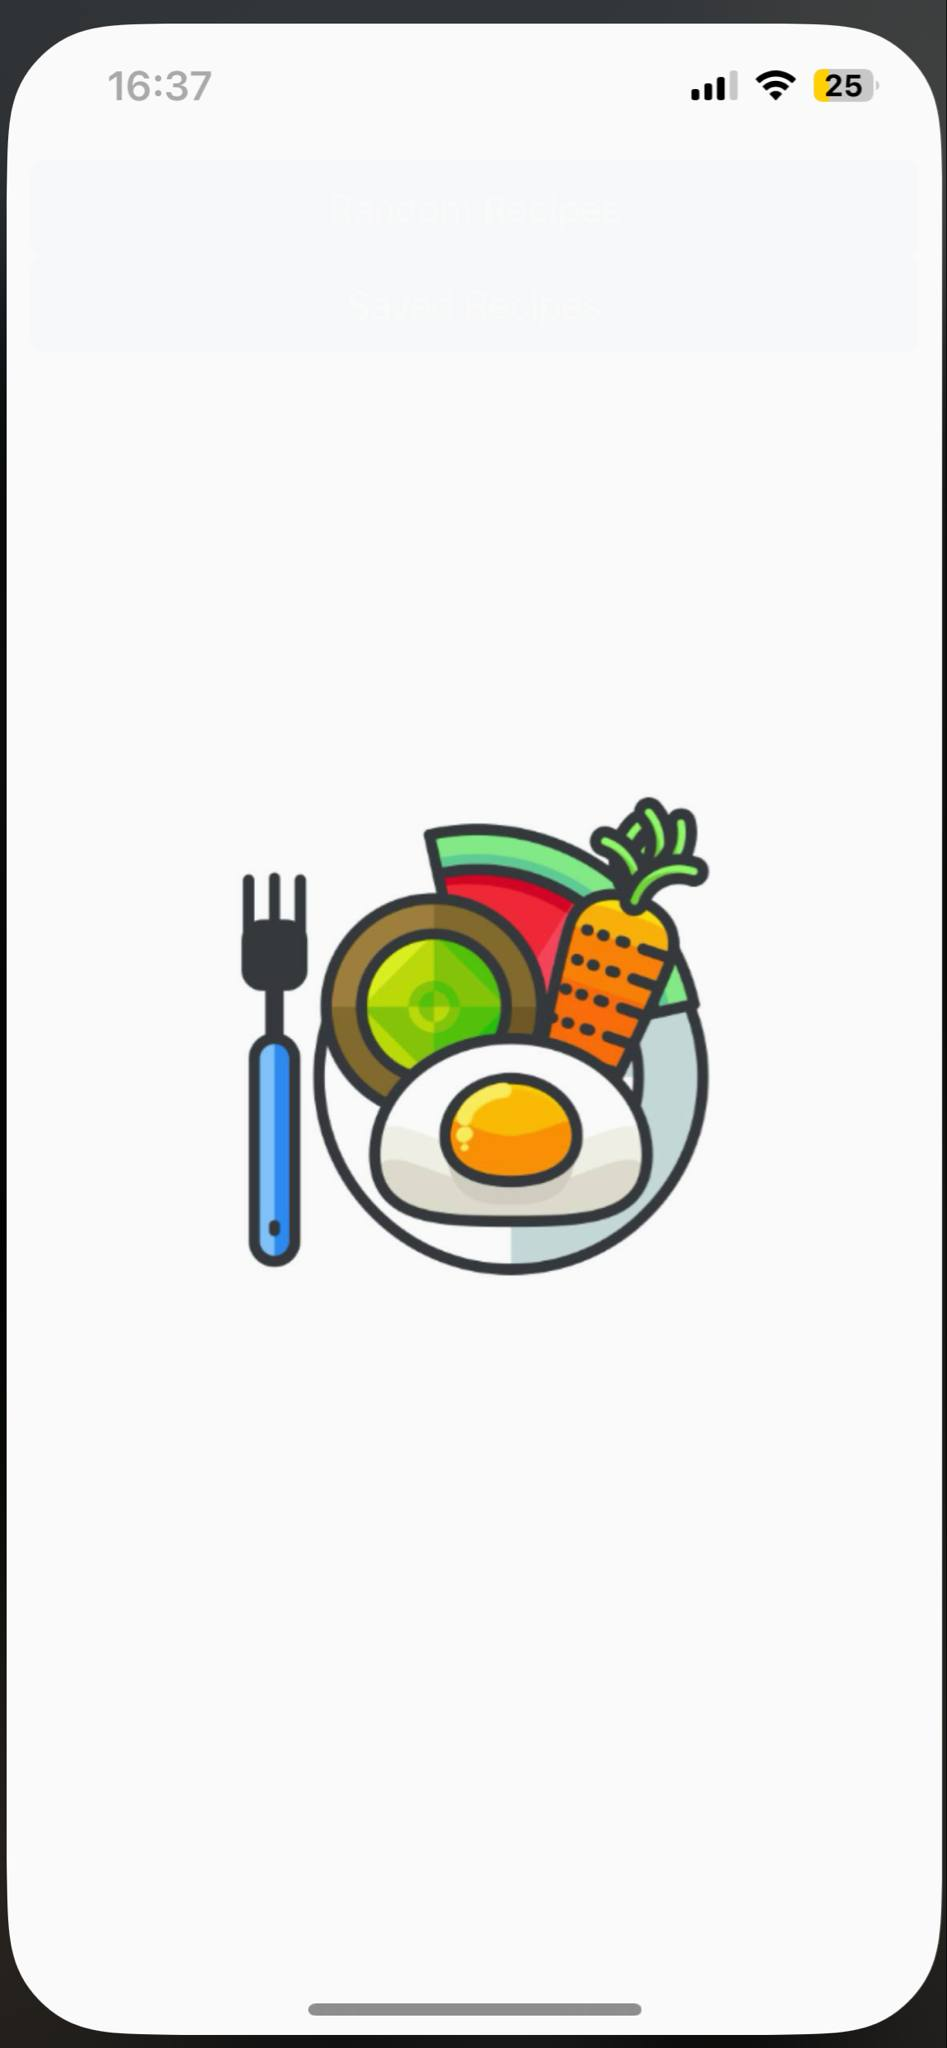
\includegraphics[width=0.3\textwidth]{images/splash.jpg}
    \caption{Splash screen}
    \label{fig:splash}
\end{figure}

\begin{figure}[H]
    \centering
    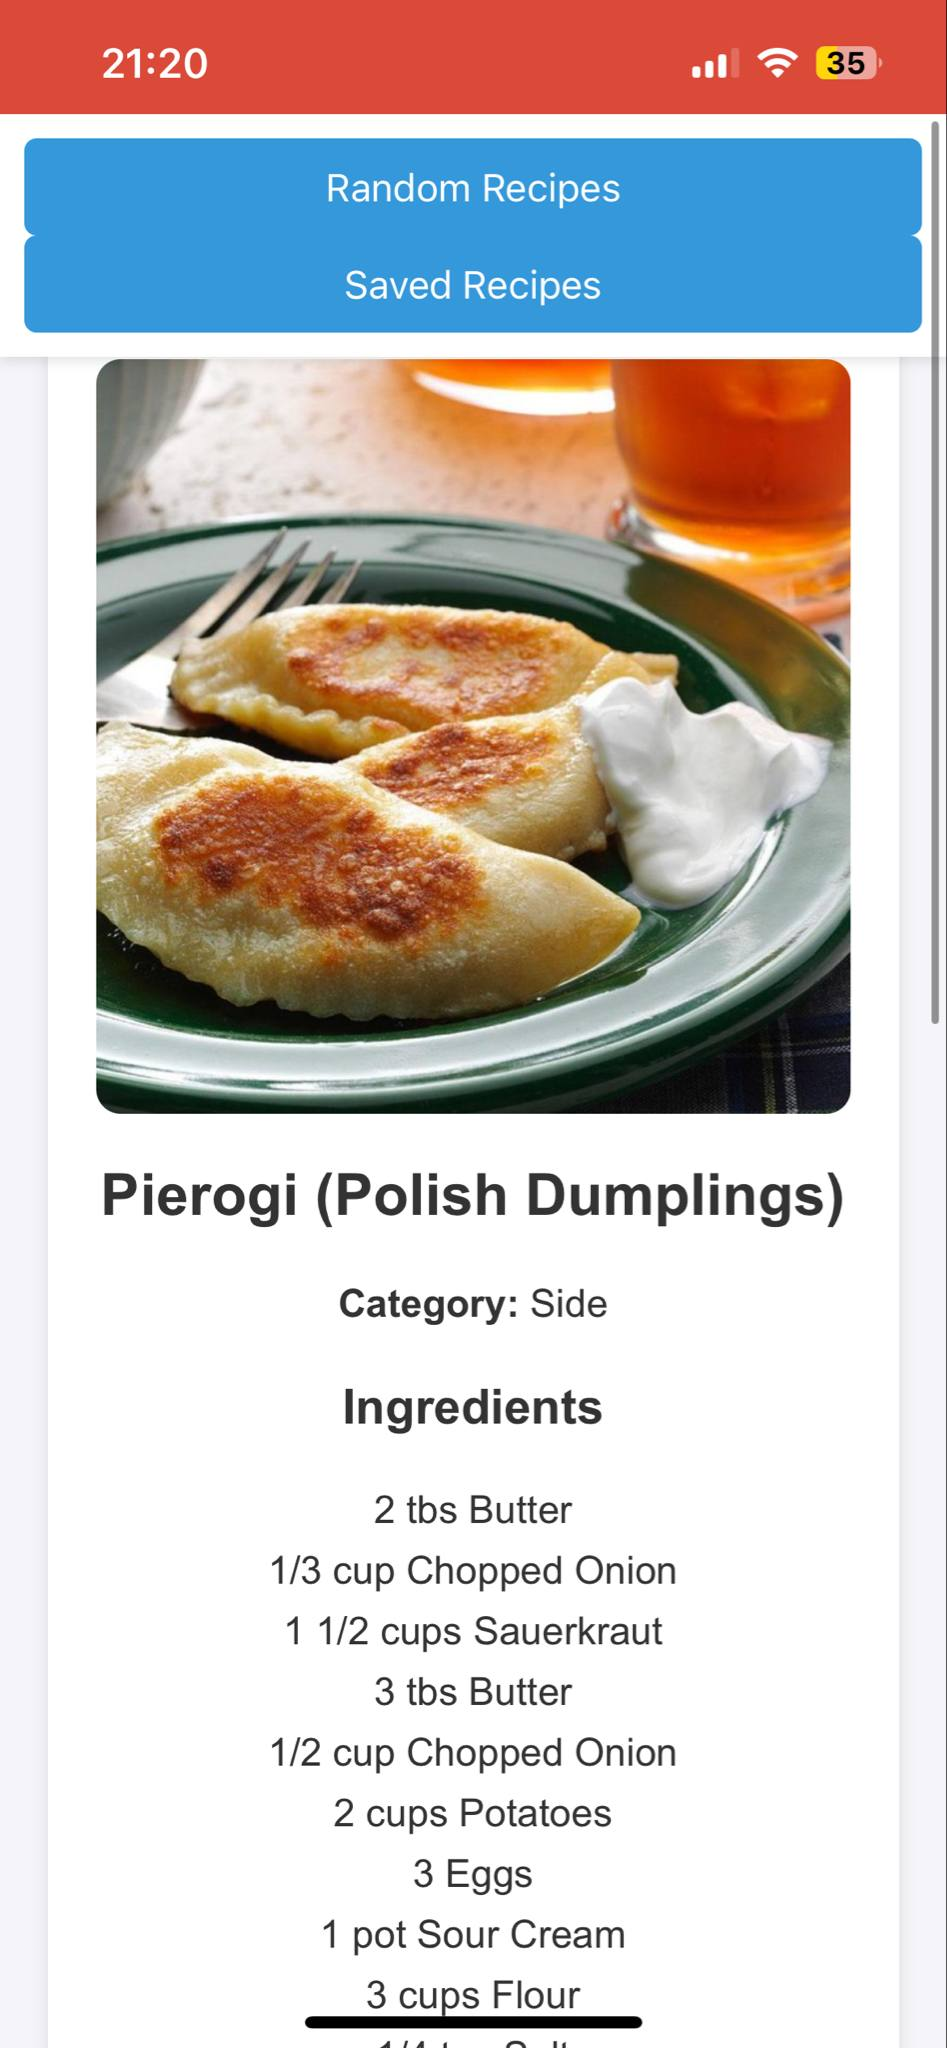
\includegraphics[width=0.3\textwidth]{images/losowy.jpg}
    \caption{Losowy przepis}
    \label{fig:random}
\end{figure}

Jeśli nie ma dostępu do internetu, aplikacja umożliwia tylko przeglądanie ulubionych przepisów.

\begin{figure}[H]
    \centering
    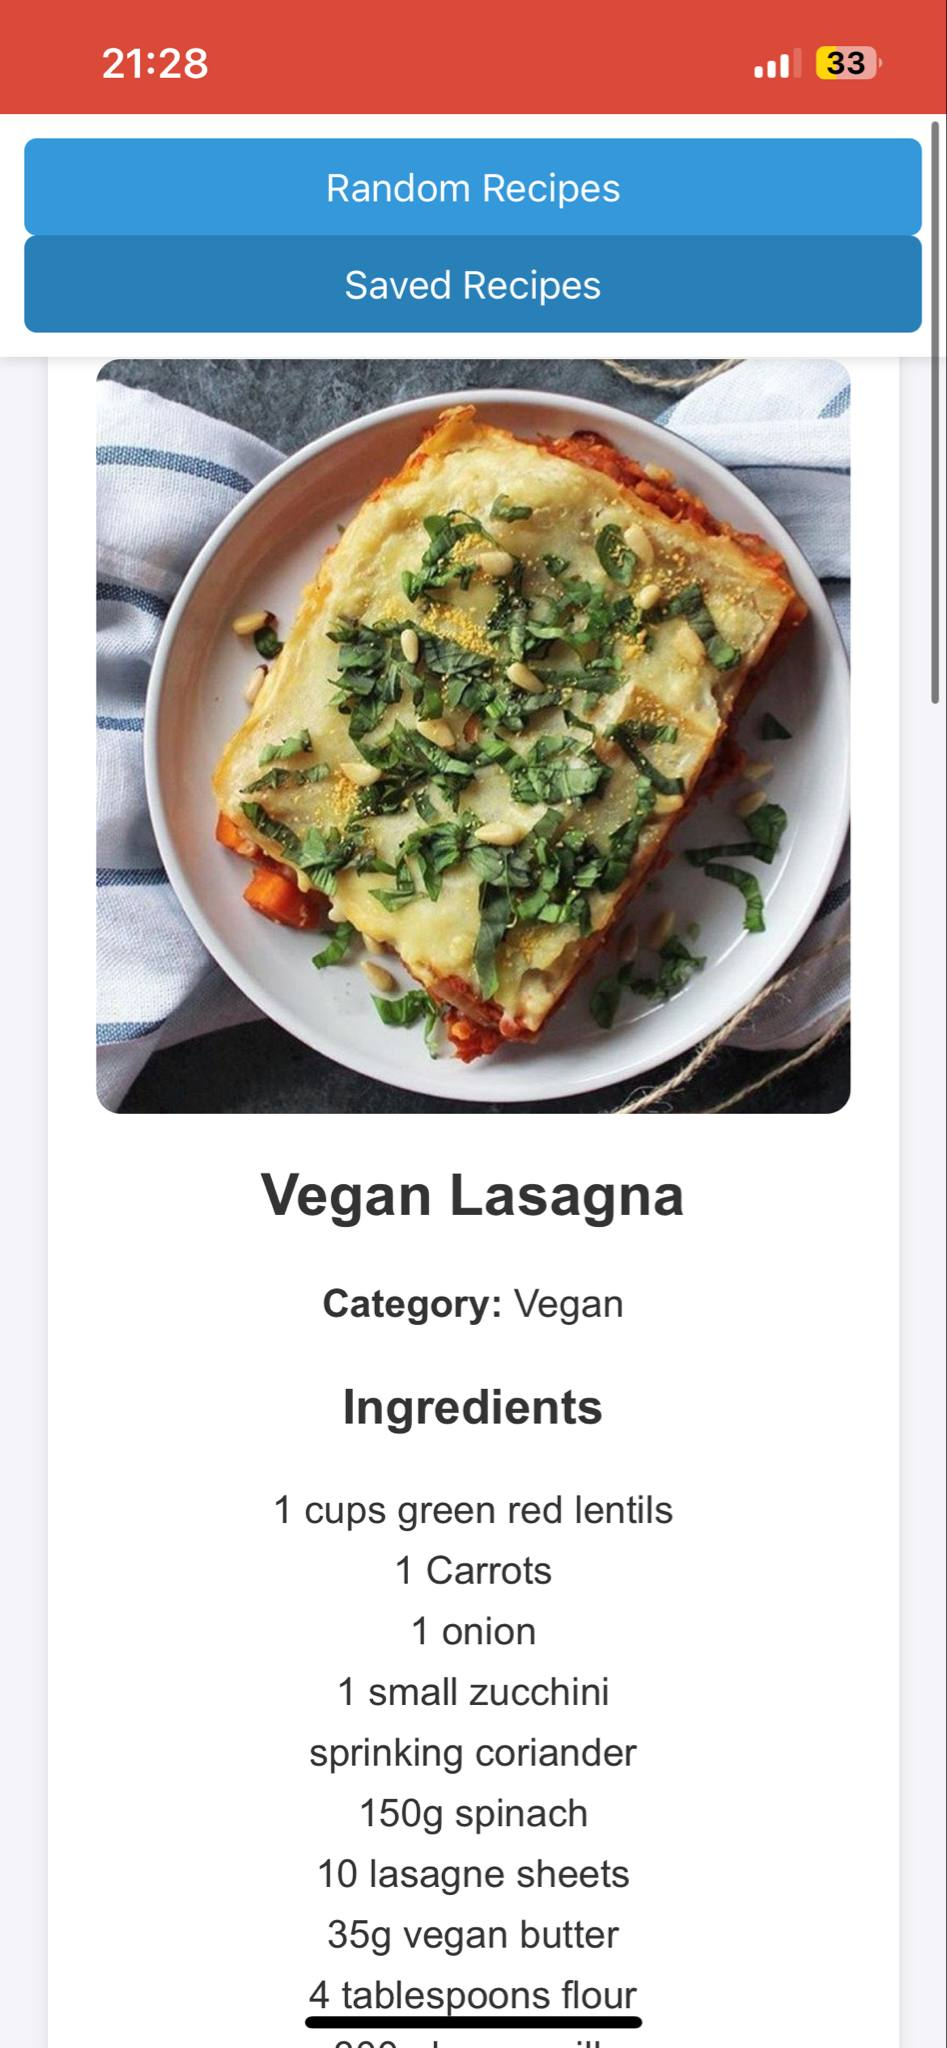
\includegraphics[width=0.3\textwidth]{images/zapisany.jpg}
    \caption{Losowy przepis}
    \label{fig:saved}
\end{figure}

W przypadku urządzeń z systemem iOS istnieje łatwy sposób "zainstalowania" takiej aplikacji, co też zostało przetestowane, a wszystkie screeny pochodza właśnie z tak pobranej aplikacji.

\begin{figure}[H]
    \centering
    
\includegraphics[width=0.3\textwidth]{images/ikona.jpg}
    \caption{Aplikacja pobrana na iOS}
    \label{fig:ios}
\end{figure}

\section{Wdrożenie aplikacji}
Aplikacja została wdrożona na platformie GitHub Pages. Nie sprawiało to żadnych problemów, oprócz potrzeby zmian linków, aby odwzorowały poprawną lokalizację plików.

\begin{figure}[H]
    \centering
    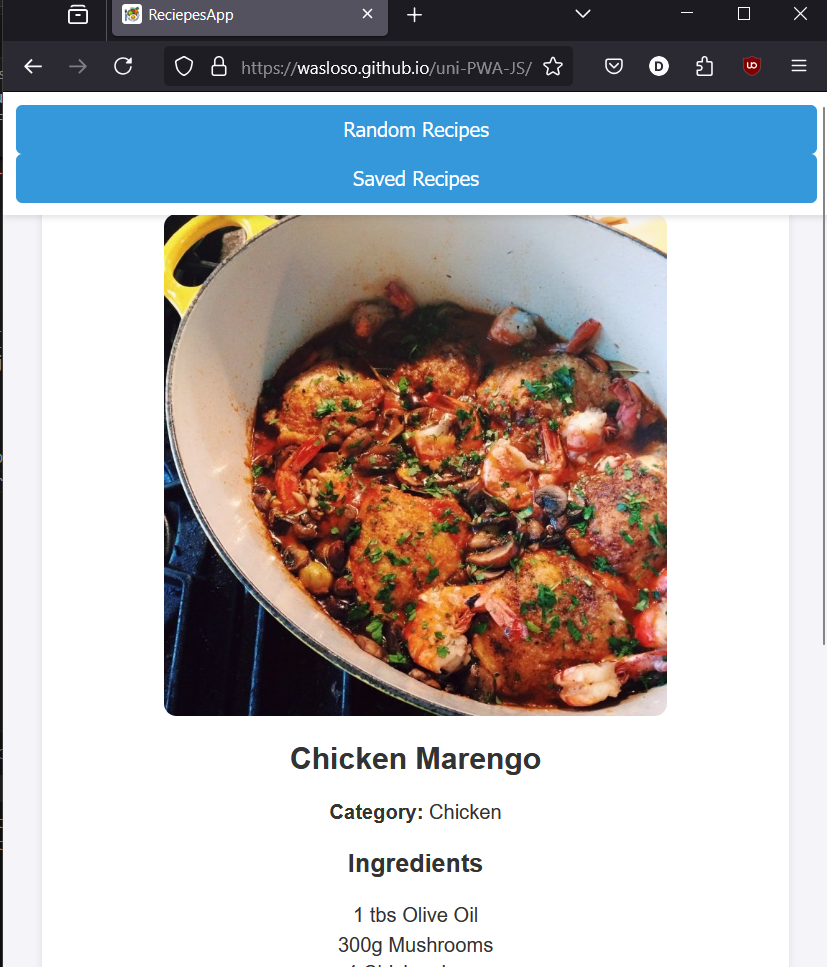
\includegraphics[width=0.5\textwidth]{images/gp.png}
    \caption{Aplikacja wdrożona na GitHub Pages}
    \label{fig:gp}
\end{figure}

\end{document}